%\section{Introductory concepts in Quantum Chemistry} \label{sec:intro_q_chem}

%\subsection{The Hartree-Fock (HF) method} \label{sec:hartree-fock}

%The Hartree-Fock (HF) method \cite{Hartree1928, Slater1928, Gaunt1928, Hartree1935, Jensen2017} gives a first approximation of the ground state molecular wavefunction, as well as being a usual starting point for more accurate approximations. It is a mean field method, in that it treats a multi-particle problem as a single particle problem averaging the electron-electron interaction. 

%The method starts from the assumption that the electronic wavefunction has the form of a Slater determinant as given by Eq. (\ref{eq:slaterdeterminant}). The goal of the Hartree-Fock method is to find an expression for the molecular orbitals $\{ \Phi_i(\mathbf{x}) \}$ as linear combinations of a given set of basis functions $\{ \chi_j(\mathbf{x}) \}$ (conventionally called atomic orbitals: these could be for instance hydrogen-like wavefunctions), thus giving the Slater determinant that best approximates the ground state for a given set of basis functions
%\begin{equation}
%\Phi_i(\mathbf{r}) = \sum_j U_{ij} \chi_j(\mathbf{r}).
%\end{equation}
%That is, given a basis set of atomic orbitals $\{ \chi_j(\mathbf{r}) \}$, the Hartree-Fock method gives us the unitary matrix, with coefficients $U_{ij}$ that define the molecular orbitals $\{ \Phi_i(\mathbf{r})\}$ (which we can again split in a set of spin-orbitals $\{ \phi_i(\mathbf{x})\}$, $x = \{\mathbf{r}, \sigma \}$ with $\sigma$ the spin). The requirement that the wavefunction should be of the form of a single Slater determinant is equivalent to the requirement that the electron-electron interaction is only taken into account as a mean-field interaction: in Hartree-Fock we only assumes an average repulsion between electrons. 

%We first define the Fock operator, which only includes one body term. It is a simplified version of the Hamiltonian of Eq. (\ref{eq:molecularhamiltonianladder}) that turns it into a sum of one-electron operators of the form
%\begin{equation}
%\label{eq:fockoperator1}
%\hat{F} =\sum_{p q} f_{p q} \hat{a}_{p}^{\dagger} \hat{a}_{q},
%\end{equation}
%where:
%\begin{equation}
%\label{eq:fockoperator2}
%f_{p q} = h_{p q} + \sum_{k} \left( 2 h_{p q k k} - \sum_{k} h_{p k k q} \right),
%\end{equation}
%with the indexed $h$ defined as the one and two body integrals from Eq. (\ref{eq:HFintegral1}) and Eq. (\ref{eq:HFintegral2}) respectively. At this stage, these are unknown and can be formulated from an initial guess on the composition of the molecular orbitals. The first term ($h_{pq}$ corresponds to the kinetic energy of the electron and its Coulomb attraction to the nucleus. The second term is given by the Coloumb interaction with the other electrons and is in turn made up of two different kinds of terms: those corresponding to the classical Coulomb interaction ($h_{p q k k}$) and the purely quantum mechanical exchange potential terms ($h_{p k k q}$).

%The Fock operator can be derived by imposing the variational constraint of finding the single Slater determinant corresponding to the lowest energy by optimizing the coefficients $U_{ij}$. A set of orbitals $\{ \phi_i(\mathbf{x}) \}$ whose antisymmetrised product gives this Slater determinant are the eigenfunctions of the Fock operator
%\begin{equation}
%\label{eq:fockoperator3}
%\hat{F}\phi_i = \epsilon_i \phi_i
%\end{equation}
%This is called a pseudo-eigenvalue equation because unlike a usual eigenvalue equation, the Fock operator $\hat{F}$ is constructed from the integrals of Eq. (\ref{eq:HFintegral1}) and Eq. (\ref{eq:HFintegral2}) in terms of its own eigenfunctions. The objective of the Hartree-Fock method is to find a self-consistent solution for this equation. A tentative Fock operator $\hat{F}^{(0)}$ is initially constructed from an initial guess of the orbitals $\{ \phi^{(0)}_i(\mathbf{x}) \}$ and then updated iteratively to a new operator $\hat{F}^{(j)}$ by performing each time the integrals of Eq. (\ref{eq:HFintegral1}) and Eq. (\ref{eq:HFintegral2}), which is then diagonalized to give a new set of of orbital functions $\{ \phi^{(j)}_i(\mathbf{x}) \}$. This process is repeated until convergence is obtained, yielding the final set of orbitals $\{ \phi_i(\mathbf{x}) \}$, which are self-consistent in the sense that they satisfy Eq. (\ref{eq:fockoperator3}). 

%The main advantage of the Hartree-Fock method is its relatively low computation cost. Its most basic implementation scales $\mathcal{O}(n^4)$ in the number of basis functions, although more efficient implementations can significantly reduce cost and scaling for larger system \cite{Koppl2016}. The method however fails to capture accurately energy resulting from electron-electron repulsion (the electron correlation energy), which can result in large errors for many systems. As such it is often used as a starting point for an initial estimates of the electron wavefunction and ground energy, on which more advanced can be constructed (usually named post-Hartree-Fock methods, or electron correlation methods \cite{Jensen2017}). 

%\subsection{The Hubbard model} \label{sec:hubbard}

%The Hubbard model is a central example of lattice model, used for example to describe itinerant ferromagnetism in transition metals like iron and nickel find in most common magnets, where interacting electrons wander through the lattice of atoms and are responsible at the same time for the conductive and magnetic properties of the material \cite{Simon2013}. To present the Hubbard model, we can first consider the simpler tight binding model, used to describe electronic band structure, where the approximate Hamiltonian is given in the second quantization formalism by
%\begin{equation}
%\label{eq:tightbinding}
%\hat{H} = t \sum_{<p, q>} ( \hat{a}_{p}^{\dagger} \hat{a}_{q} + \hat{a}_{q}^{\dagger} \hat{a}_{p})
%\end{equation}
%where the sum is only taken for neighboring lattice sites and for spins that are aligned, and the term $t$ is called the hopping term and gives the amplitude of an electron tunneling from one lattice site to an adjacent side. The Hubbard model generalizes this approach by adding an extra term to the Hamiltonian
%\begin{equation}
%\label{eq:Hubbardmodel}
%\hat{H} = t \sum_{<p, q>} ( \hat{a}_{p}^{\dagger} \hat{a}_{q} + \hat{a}_{q}^{\dagger} \hat{a}_{p}) + U \sum_{p} \hat{a}_{2p}^{\dagger} \hat{a}_{2p + 1}^{\dagger} \hat{a}_{2p} \hat{a}_{2p + 1},
%\end{equation}
%where we have taken even indices to correspond to electrons with spins in one direction and odd indices to correspond to electrons with spins in the opposite direction, so that the $2p$-th and the $2p + 1$-th fermionic operators create electrons of opposite spin on the same site. The first term in Eq. (\ref{eq:Hubbardmodel}) is the tight binding Hamiltonian, and the second term is the Hubbard interaction term which gives an energy penalty of $U$ whenever two electrons are found on the same lattice site. The Hubbard model Hamiltonian is a special case of the molecular Hamiltonian given by Eq. (\ref{eq:molecularhamiltonianladder}), where the only nonzero one-electron terms are the ones in between adjacent sites with the same spin and are all equal, and the only nonzero two-electron terms are the ones corresponding to the Coulomb repulsion between terms on the same lattice site and are all equal.

\section{Qubit encodings and Fenwick trees} \label{sec:Fenwick_trees}

The qubit encondings that have been presented in Sec. \ref{sec:gen_encoding} can be translated into the language of graph theory and be visualized in a simple way as Fenwick trees \cite{Havlek2017}.
\begin{figure}
\centering
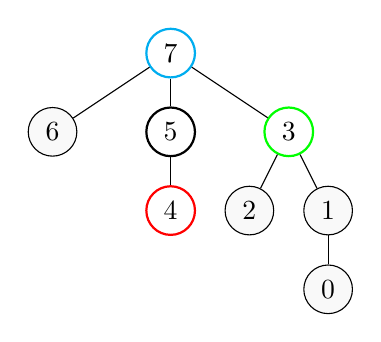
\begin{tikzpicture}
\node[shape=circle,fill=white,thick,draw=cyan] (7) at (0,0) {7};  \node[shape=circle,draw=black,fill=gray!5] (6) at (-1.5,-1) {6};
\node[shape=circle,draw=black,fill=white, thick] (5) at (0,-1) {5};
\node[shape=circle,fill=white,thick,draw=red] (4) at (0,-2) {4};
\node[shape=circle,fill=white,thick,draw=green] (3) at (1.5,-1) {3};
\node[shape=circle,draw=black,fill=gray!5] (2) at (1,-2) {2};
\node[shape=circle,draw=black,fill=gray!5] (1) at (2,-2) {1};
\node[shape=circle,draw=black,fill=gray!5] (0) at (2,-3) {0};

\path [-] (6) edge (7);
\path [-] (5) edge (7);
\path [-] (3) edge (7);
\path [-] (4) edge (5);
\path [-] (2) edge (3);
\path [-] (1) edge (3);
\path [-] (0) edge (1);
\end{tikzpicture}
\caption{Fenwick tree for the Bravyi-Kitaev encoding of 8 qubits showing the update set $U(5) = \{7\}$ (cyan), flip set $F(5) = \{4\}$, (red) and remainder set $R(5) = \{3\}$ (green) for qubit $5$, from which we can read off the Brayvi-Kiteav operators (See Sec. \ref{sec:bravyi-kitaev})}
\label{fig:BK8qubit-5}
\end{figure}
The tree corresponding to the Bravyi-Kitaev (like the one shown in Fig. (\ref{fig:BK8qubit-5}) and in Fig (\ref{fig:BK8qubit-2})) can be built recursively according to a procedure that mirrors the construction of the change of basis matrix of Eq. (\ref{eq:bravyikitaev2}): the tree corresponding to the single-qubit encoding is the trivial graph, and the tree corresponding to the $2^x$-qubit enconding is built from two copies of the tree corresponding to the $2^{x-1}$-qubit enconding, where vertex $k$ on the first tree corresponds to vertex $k + 2^{x-1}$ on the second, and the two trees are joined together by making vertex $2^{x-1} - 1$ a child of vertex $2^x  - 1$.
\begin{figure}
\centering
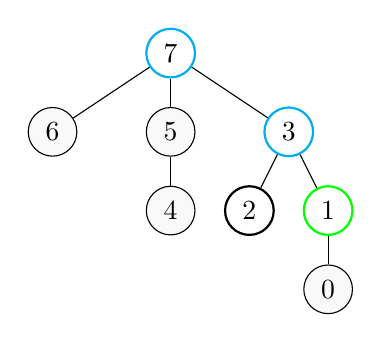
\begin{tikzpicture}
\node[shape=circle,fill=white,thick,draw=cyan] (7) at (0,0) {7};  \node[shape=circle,draw=black,fill=gray!5] (6) at (-1.5,-1) {6};
\node[shape=circle,draw=black,fill=gray!5] (5) at (0,-1) {5};
\node[shape=circle,draw=black,fill=gray!5] (4) at (0,-2) {4};
\node[shape=circle,fill=white,thick,draw=cyan] (3) at (1.5,-1) {3};
\node[shape=circle,draw=black,fill=white, thick] (2) at (1,-2) {2};
\node[shape=circle,fill=white,thick,draw=green] (1) at (2,-2) {1};
\node[shape=circle,draw=black,fill=gray!5] (0) at (2,-3) {0};

\path [-] (6) edge (7);
\path [-] (5) edge (7);
\path [-] (3) edge (7);
\path [-] (4) edge (5);
\path [-] (2) edge (3);
\path [-] (1) edge (3);
\path [-] (0) edge (1);
\end{tikzpicture}
\caption{The same Fenwick tree as in Fig. (\ref{fig:BK8qubit-5}), this time showing the update set $U(2) = \{3, 7\}$ (cyan) and remainder set $R(2) = P(2) = \{1\}$ (green) for qubit $2$ (because of how the Bravyi-Kitaev tree is constructed the leaves are the even vertices and so we see again that the flip set of an even qubit is always empty$F(2) = \emptyset$)}
\label{fig:BK8qubit-2}
\end{figure}

The definitions of the qubit sets given when describing the Bravyi-Kitaev encoding (see Sec. \ref{sec:bravyi-kitaev}) now translate into the following simple statements about Fenwick trees \cite{Havlek2017}:
\begin{itemize}
\item The update set of the $j$-th qubit $U(j)$ corresponds then to the set of ancestors of vertex $j$ on the tree.
\item The flip set $F(j)$ is the set of children of the $j$-th vertex.
\item The remainder set $R(j)$ is the set of children of the ancestors of vertex $j$ whose values is less than $j$.
\end{itemize}
This construction allows us to read off qubits sets for each qubit from the tree corresponding to our encoding (as shown in Fig. (\ref{fig:BK8qubit-5}) and in Fig (\ref{fig:BK8qubit-2}) for our usual examples of qubits 2 and 5) and hence the representation of the creation and annihilation operators using Eq. (\ref{eq:BKladder4}). In the case where the number of qubits $n$ is not a power of $2$ we construct the Fenwick tree for the next power of $2$ and determine the qubit sets, and then we discard from the qubit sets all the qubits greater or equal to $n$.

The parity encoding can also be represented this way, giving rise to the linear graph in Fig. \ref{fig:JW8qubit-5}. We can further generalize this to other encodings by considering disconnected Fenwick trees. We can then change our definition of $R(j)$ to include both the children of vertex $j$'s ancestors and the roots whose value is less than $j$. We then have that the Jordan-Wigner encoding corresponds to a totally disconnected graph (a graph with no edges). In the case of both encodings inspection of the corresponding Fenwick tree together with Eq. (\ref{eq:BKladder4}) recovers the same representations of $\hat{a}^\dagger_j$ and $\hat{a}_j$ operators as in Eq. (\ref{eq:parityladder2}) and Eq. (\ref{eq:JW2}). We can turn this argument upside down, and define new fermionic encodings starting from collections of Fenwick trees \cite{Havlek2017}.

\begin{figure}
\centering
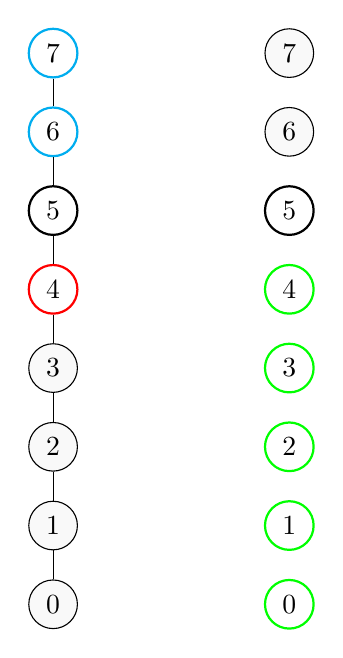
\begin{tikzpicture}
\node[shape=circle,fill=white,thick,draw=cyan] (7) at (0,0) {7};  \node[shape=circle,fill=white,thick,draw=cyan] (6) at (0, -1) {6};
\node[shape=circle,draw=black,fill=white,thick] (5) at (0, -2) {5};
\node[shape=circle,draw=red,fill=white,thick] (4) at (0, -3) {4};
\node[shape=circle,draw=black,fill=gray!5] (3) at (0, -4) {3};
\node[shape=circle,draw=black,fill=gray!5] (2) at (0, -5) {2};
\node[shape=circle,draw=black,fill=gray!5] (1) at (0, -6) {1};
\node[shape=circle,draw=black,fill=gray!5] (0) at (0, -7) {0};
\path [-] (7) edge (6);
\path [-] (6) edge (5);
\path [-] (5) edge (4);
\path [-] (4) edge (3);
\path [-] (3) edge (2);
\path [-] (2) edge (1);
\path [-] (1) edge (0);

\node[shape=circle,draw=black,fill=gray!5] (7) at (3,0) {7};  \node[shape=circle,draw=black,fill=gray!5] (6) at (3, -1) {6};
\node[shape=circle,draw=black,fill=white,thick] (5) at (3, -2) {5};
\node[shape=circle,draw=green,fill=white,thick] (4) at (3, -3) {4};
\node[shape=circle,draw=green,fill=white,thick] (3) at (3, -4) {3};
\node[shape=circle,draw=green,fill=white,thick] (2) at (3, -5) {2};
\node[shape=circle,draw=green,fill=white,thick] (1) at (3, -6) {1};
\node[shape=circle,draw=green,fill=white,thick] (0) at (3, -7) {0};
\end{tikzpicture}
\caption{Fenwick trees for the parity (left) and Jordan-Wigner (right) encoding of 8 qubits showing update $U(5)$ (cyan), flip $F(5)$ (red) and remainder sets $R(5)$ (green) for qubit 5}
\label{fig:JW8qubit-5}
\end{figure}


\section{Hadamard test}\label{sec:hadamard-test}


Here we briefly introduce a common quantum subroutine called the Hadamard test \cite{nielsenQuantumComputationQuantum2010}. Hadamard test is frequently used to compute the amplitude $\langle \psi |U|\psi \rangle $ (both its real and imaginary part) of an initial state $|\psi \rangle $ and a unitary gate $U$. This algorithm is summarized in the circuit diagram in Fig.~\ref{fig:hadamard-test}. Here we explain the circuit in detail. To measure the real part of the amplitude, the quantum computer is initialized in a product state $|\psi \rangle \otimes |0\rangle $ with one ancilla qubit. The Hadamard gate $\Had$ converts the ancilla from $|0\rangle $ to $( |0\rangle +|1\rangle ) /\sqrt{2}$. Then the controlled-$U$ gate with control qubit on the ancilla results in the state $( U|\psi \rangle \otimes |1\rangle +|\psi \rangle \otimes |0\rangle ) /\sqrt{2}$. The second Hadamard gate gives the state $(( I+U) |\psi \rangle \otimes |0\rangle +( I-U) |\psi \rangle \otimes |1\rangle ) /2$. In the final measurement, the probability of obtaining $0$ is $( 1+\mathrm{Re} \langle \psi |U|\psi \rangle ) /2$, and the probability of obtaining $1$ is $( 1-\mathrm{Re} \langle \psi |U|\psi \rangle ) /2$. Therefore, the difference between the two probabilities is $\mathrm{Re} \langle \psi |U|\psi \rangle $. Similarly calculation shows that in the second circuit (Fig.~\ref{fig:hadamard-imag}), the probability of obtaining 0 minus the probability of obtaining 1 is $\mathrm{Im} \langle \psi |U|\psi \rangle $.

\begin{figure} [ht]
  \centering
  \subfloat[$\mathrm{Re}\langle \psi | U | \psi \rangle$\label{fig:hadamard-real}]{
  \Qcircuit @C=1.0em @R=0.2em @!R { 
     \nghost{ |0\rangle  } & \lstick{ |0\rangle } & \gate{\Had} & \ctrl{1} & \gate{\Had} & \meter & \cw\\ 
     \nghost{ |\psi\rangle } & \lstick{ |\psi\rangle } & {/} \qw & \gate{U} & \qw & \qw & \qw \\ 
  }
  }
  \subfloat[$\mathrm{Im}\langle \psi |U|\psi\rangle$\label{fig:hadamard-imag}]{
  \Qcircuit @C=1.0em @R=0.2em @!R { 
     \nghost{ |0\rangle  } & \lstick{ |0\rangle } & \gate{\Had} & \gate{\mathrm{Rz}(-\frac{\pi}{2})} & \ctrl{1} & \gate{\Had} & \meter & \cw\\ 
     \nghost{ |\psi\rangle } & \lstick{ |\psi\rangle } & {/} \qw & \qw & \gate{U} & \qw & \qw & \qw \\ 
  }
  }
  \caption{
  Hadamard test circuits. The probability of measuring $0$ minus the probability of measuring
  $1$ in \protect\subref{fig:hadamard-real} and \protect\subref{fig:hadamard-imag} 
  gives respectively the real the imaginary part of the amplitude
  of $\langle \psi|U|\psi \rangle$.
  }
  \label{fig:hadamard-test}
\end{figure}


\section{Error mitigation appendix}
\subsection{Common noise models} \label{sec:common_noise_models}
Here we mention a few noise models that may be common in the literature, as for most relevant concepts in quantum computing, readers can refer to Ref.~\cite{nielsenQuantumComputationQuantum2010} for further details.

\subsubsection{Relaxation rates}
\label{sec:mit-noise-relaxation}

We start with the $T_1$ and $T_2$ relaxation time of a quantum computer. They are commonly used as a figure of merit for the noise robustness of a quantum computer. $T_1$ and $T_2$ captures the error on a single qubit quantum state $\rho$ due to thermalization to an equilibrium state with the environment. Specifically, assume the initial quantum state $\rho$ is
\begin{equation}
    \label{eq:error-mit-noise-model-rho}
    \rho = \begin{pmatrix}
        a     & b   \\
        b^{*} & 1-a
    \end{pmatrix}.
\end{equation}
Then, after a period of time $t$, the quantum state is changed by the noise $\mathcal{N}$ into~\cite{nielsenQuantumComputationQuantum2010}

\begin{equation}
    \mathcal{N}(\rho) = \begin{pmatrix}
        ( a-a_{0}) e^{-t/T_{1}} +a_{0} & be^{-t/T_{2}}                     \\
        b^{*} e^{-t/T_{2}}             & ( a_{0} -a) e^{-t/T_{1}} +1-a_{0}
    \end{pmatrix},
\end{equation}
where $a_{0}$ represents the thermal equilibrium state, and usually $a_{0}=1$ on superconducting qubits.
The parameters $T_{1}$ and $T_2$ are also known as spin–lattice (or `longitudinal') and spin–spin (or `transverse') relaxation rates. They can be obtained experimentally are widely available metrics for most quantum computers today.

\subsubsection{Over-rotation}

This type of error happens when a physical pulse used to generate a particular gate are mis-calibrated
\cite{merrillProgressCompensatingPulse2012}. In the case or Pauli rotation gates $R_{i}(\theta)$, $i\in\{x,y,z\}$,
this error manifests a small deviation $\delta$ in the angle $\theta$, resulting in an actual gate of modified
rotation gate $R_i(\theta + \delta)$. The deviation may be systematic\cite{bultriniSimpleMitigationStrategy2020}, but may also be stochastic and usually varies differently from different quantum computer.


\subsubsection{Depolarizing noise model}

The depolarizing model $\mathcal{N}_{\text{depolar}}$ is a common noise model. On a quantum state $\rho$ of $n$ qubits, it changes $\rho$ according to

\begin{equation}
    \mathcal{N}_{\text{depolar}}( \rho ) =( 1-\varepsilon ) \rho +\varepsilon \frac{\unit{}}{2^{n}},
\end{equation}
where $\unit{}$ is the identity matrix on $n$ qubits, and $\varepsilon$ characterizes the strength of the depolarizing noise.

\subsubsection{Dephasing noise model}

The dephasing noise model $\mathcal{N}_{\mathrm{dephasing}}$ is related to the disappearance of off-diagonal part of a density matrix, hence closely related to the $T_2$ relaxation rate of a quantum computer. Its action on a single qubit state $\rho$ is described by

\begin{equation}
    \begin{aligned}
        \mathcal{N}_{\mathrm{dephasing}}(\rho ) & =( 1-\varepsilon ) \rho +\varepsilon Z\rho Z \\
                                                & =\left(\begin{array}{ c c }
                a                       & b( 1-2\varepsilon ) \\
                b^{*}( 1-2\varepsilon ) & 1-a
            \end{array}\right),
    \end{aligned}
\end{equation}
where $a$ and $b$ characterize the initial state of $\rho$ (Eq.~\ref{eq:error-mit-noise-model-rho}), $\varepsilon$ characterizes the strength of this noise model. It's clear that the depolarizing noise does not affect the diagonal part of a single qubit state, therefore it commutes with most symmetry operator and could not be detected by the symmetry verification technique mentioned in Sec.~\ref{sec:mit-symmetry-verification}.

\subsubsection{Damping error}

Here as suggested by the name, the damping error decreases the population of $\ket{1}$ in a single qubit state, and is closely related to the $T_1$ relaxation time.
This error model can be described by the Kraus operators
\begin{equation}
    K_{0} =\begin{pmatrix}
        1 & 0                     \\
        0 & \sqrt{1-\varepsilon }
    \end{pmatrix},\;
    K_{1} =\begin{pmatrix}
        0 & 0                   \\
        0 & \sqrt{\varepsilon }
    \end{pmatrix},
\end{equation}
where $\varepsilon$ characterizes the strength of this noise model. Its action on the initial state $\rho$ in Eq.~(\ref{eq:error-mit-noise-model-rho}) is

\begin{equation}
    \begin{split}
        & \mathcal{N}_{\mathrm{damping}}(\rho) = \sum_{i=0}^1 K_i \rho K_i^\dagger \\
        & = \begin{pmatrix}
            1+(a-1)(1-\varepsilon )    & b\sqrt{1-\varepsilon } \\
            b^{*}\sqrt{1-\varepsilon } & (1-a)(1-\varepsilon )
        \end{pmatrix}.
    \end{split}
\end{equation}

\subsection{Example for probabilistic error cancellation}
\label{sec:mit-pec-toy-example}

Here we present an illustrative example of using probabilistic error cancellation to correct the depolarizing error on a one-qubit quantum computer. The depolarizing noise $\mathcal{N}_{\mathrm{dep}}$ changes an initial state $\rho$ to

\begin{equation}
    \label{eq:mit-pec-2}
    \mathcal{N}_{\mathrm{dep}}( \rho ) =\left( 1-\frac{3}{4} p\right) \rho +\frac{p}{4}\sum _{\sigma \in \{X,Y,Z\}} \sigma \rho \sigma .
\end{equation}
Here $p\in \left[ 0,\frac{4}{3}\right]$ characterizes the strength of the depolarizing noise, and $\{X,Y,Z\}$ are the Pauli matrices. One can show that $\mathcal{N}^{-1}_{\mathrm{dep}}$ can be written as~\cite{temmeErrorMitigationShortDepth2017}

\begin{equation}
    \label{eq:mit-pec-3}
    \begin{split}
        \mathcal{N}^{-1}_{\mathrm{dep}}( \rho ) & =\gamma _{\mathrm{PEC} ,\ \mathrm{dep}}\left( q_{\mathrm{dep} ,1} \rho +q_{\mathrm{dep} ,2}\sum _{\sigma \in \{X,Y,Z\}} \sigma \rho \sigma \right) ,\\
        \gamma _{\mathrm{PEC} ,\ \mathrm{dep}} & =\frac{p+2}{2-2p} ,\\
        q_{\mathrm{dep} ,1} & =\frac{4-p}{2p+4} ,\\
        q_{\mathrm{dep} ,2} & =-\frac{p}{2p+4} .
    \end{split}
\end{equation}

Suppose the effective quantum channel of an ideal unitary $U$ on quantum computer could be characterized as $\mathcal{N}_{1} \circ U$, where the circle $\circ $means composition of quantum channels. One could define three additional quantum circuits, each formed by appending one of the three Pauli gates after the unitary $U$.
One obtains the measurement outcome from the four circuits $\{U,X\circ U,Y\circ U,Z\circ U\}$ containing the original one, and calculates according to the weights in Eq.~(\ref{eq:mit-pec-3})

\begin{equation}
    \begin{split}
        \label{eq:mit-pec-4}
        & \langle \hat{O} \rangle_{\mathrm{PEC} ,\ \mathrm{dep}}                                                                                                                                                \\
        = & \gamma _{\mathrm{PEC} ,\ \mathrm{dep}}\bigg(q_{\mathrm{dep} ,1}\underbrace{\operatorname{Tr}[\hat{O} \mathcal{N}_{1} \circ U( \rho )]}_{\text{original circuit}} + q_{\mathrm{dep} ,2}\sum _{\sigma \in \{X,Y,Z\}}\underbrace{\operatorname{Tr}[ \hat{O} \sigma \circ \mathcal{N}_{1} \circ U( \rho )]}_{\text{appended by a Pauli gate}}\bigg)               \\
        = & \operatorname{Tr}\Big[\hat{O}\underbrace{\mathcal{N}^{-1}_{1}(\mathcal{N}_{1} \circ U( \rho ))}_{\text{quasi-probability\ representation\ of\ } U\ \text{acting\ on} \ \rho }\Big] \\
        = & \operatorname{Tr}[ \hat{O} U( \rho ))].
    \end{split}
\end{equation}
Therefore, the noise effect of $\mathcal{N}_{1}$ can be canceled with the PEC method.

\subsection{Implementation of exponential error suppression}
\label{sec:derangement-details}

%the first method
Here we will mention several methods to actually compute the value in Eq.~(\ref{eq:ees-computed-rhon}) using quantum computers. For simplicity, we mostly consider the computation of the numerator
\begin{equation}
    \label{eq:ees-numerator}
    \mathrm{Tr( \rho^{\nEES} \hat{O})},
\end{equation}
since the denominator is a special case of the numerator with $\hat{O}$ being the identity observable.

\subsubsection{Ancilla assisted method}
\label{sec:derangement-details_ancilla-assisted}
The first method needs the assistance of an extra ancilla qubits. Considering
$n$ copies of the same state $\rho^{\otimes \nEES}$. We want to measure the observable $O$ only on one system, but
in as an overlap of the original state, and a permuted state. Specifically, we want to compute the quantity

\begin{equation}
    \label{eq:ees-single1}
    \begin{aligned}
          & \langle \psi _{i_1} |\otimes \cdots \otimes \langle \psi _{i_n} |O^{( 1)} |\psi _{s ( i_{1})} \rangle \otimes \cdots \otimes |\psi _{s ( i_{\nEES})} \rangle \\
        = & \langle \psi _{i_{1}} |O|\psi _{i_{1}} \rangle \delta _{i_{1} ,s ( i_{1})} \cdots \delta _{i_{n} ,s ( i_{\nEES})},
    \end{aligned}
\end{equation}
where for simplicity we consider only one possibility
$|\psi _{i_1} \rangle\otimes \cdots \otimes |\psi _{i_\nEES}\rangle$ in the
statistical mixture $\rho^{\otimes \nEES}$,
$O^{(1)}$ is the same observable $O$ on any one of the $n$ copies of the same system,
$s$ is called the $\nEES$-cycle derangement in the Group theory. Explicitly, $s$ is a permutation in the indices $\{1,2,\cdots \nEES\}$, and can be written as mappings
\begin{equation}
    \label{eq:ees-VD-ncycle}
    \begin{aligned}
        s( i_{1})   & =i_{2}\\
        s( i_{2})   & =i_{3}   \\
                    & \cdots   \\
        s( i_{n-1}) & =i_{\nEES}   \\
        s( i_{n})   & =i_{1} ,
    \end{aligned}
\end{equation}
where all indices $\{i_1,\cdots,i_\nEES\}$ are distinct numbers. An example is
\begin{equation}
    \label{eq:ees-cycle-all}
    s(i) = i+1,\,(i< \nEES),\, s(\nEES) = 1.
\end{equation}

$s$ being a permutation of all indices (i.e. $\{i_1,\cdots,i_\nEES\}$ are distinct numbers above)
enforces the delta functions $\delta _{i_{1} ,s ( i_{1})} \cdots \delta _{i_{n} ,s ( i_{\nEES})}$
in Eq.~(\ref{eq:ees-single1}).
For the statistical mixture $\rho^{\otimes \nEES}$, we are effectively computing $\operatorname{Tr}[\rho^\nEES O]$ since

\begin{equation}
    \begin{aligned}
          & \sum _{i_{1} \cdots i_{n}} p_{i_{1}} \cdots p_{i_{\nEES}}                                                                                                                         \\
          & \times \langle \psi _{i_{1}} |\otimes \cdots \otimes \langle \psi _{i_{\nEES}} |O^{( 1)} |\psi _{\sigma ( i_{1})} \rangle \otimes \cdots \otimes |\psi _{\sigma ( i_{\nEES})} \rangle \\
        = & \sum _{i_{1}} p_{i_{1}}^{\nEES} \langle \psi _{i_{1}} |O|\psi _{i_{1}} \rangle =\operatorname{Tr}\left[ \rho ^{\nEES} O\right].
    \end{aligned}
\end{equation}

Given an explicit expression for $s$, it is easy to construct a circuit $D_\nEES$ which performs the unitary mapping
\begin{equation}
    |\psi _{i_1} \rangle\otimes \cdots \otimes |\psi _{i_\nEES}\rangle
    \mapsto
    |\psi _{s ( i_{1})} \rangle \otimes \cdots \otimes |\psi _{s ( i_{\nEES})} \rangle.
\end{equation}
For example, for the $s$ in Eq.~(\ref{eq:ees-cycle-all}), $D_m$ can be constructed by
performing CNOT operations on pairs of qubits $(1,2),\cdots,(\nEES-1,\nEES),(\nEES,1)$.
Having constructed $|\psi _{s ( i_{1})} \rangle \otimes \cdots \otimes |\psi _{s ( i_{\nEES})} \rangle$,
measuring the overlap in Eq.~(\ref{eq:ees-single1}) could be achieved easily with a modified
Hadamard test, which is illustrated in the circuit diagram in Fig.~\ref{fig:ees-general-circ}.

We note that several improvements of the derangement operation $D_\nEES$ exists in the literature~\cite{hugginsVirtualDistillationQuantum2021, czarnikQubitefficientExponentialSuppression2021}. In particular,
\citet{czarnikQubitefficientExponentialSuppression2021} utilize a deep circuit to achieve derangement on a single copy, avoiding creating $\nEES$ copies of $\rho$ and applying the derangement operation on all $\nEES$ copies.
Although $D_\nEES$ seems to be prone to errors on actual quantum computer due to its long-range nature,
as long as the error does not affect the orthogonal relations in Eq.~(\ref{eq:ees-single1}), the noisy $D_\nEES$
is still a valid derangement operation, and it is shown in \citet{koczorExponentialErrorSuppression2021}
that the error induced by $D_\nEES$ could be
mitigated effectively with extrapolation based mitigation techniques.


\subsubsection{Diagonalization method}
\label{sec:derangement-details_diagonalization}
In the second method, we reformulate the derangement operation
as a matrix $S$, and implement a unitary version of
$S$ and the observable after the derangement operation $OS$ in order to
estimate the denominator and the numerator of Eq.~(\ref{eq:ees-computed-rhon}).
Compared with the previous method, this method does not require additional
ancilla qubit and the long range controlled-$D_\nEES$ operation (Fig.~\ref{fig:ees-general-circ}). This method only performs local operations $B_i$ which connects the same set of qubits in each copy of the state $\rho$ in $\rho^{\otimes \nEES}$.
We will first describe a general method, and then specialize on a specific case ($\nEES=2$, $O$ acts only one qubit only)
to illustrate the potential of this method.

We can define a matrix $S$ which swaps quantum systems as defined by the derangement permutation
$s$ in Eq.~(\ref{eq:ees-VD-ncycle})
\begin{equation}
    \label{eq:ees-derangement-matrix-S}
    S | \psi _{i_1} \rangle \otimes \cdots \otimes | \psi _{i_\nEES} \rangle
    = |\psi _{s ( i_{1})} \rangle \otimes \cdots \otimes |\psi _{s ( i_{\nEES})} \rangle.
\end{equation}
It should be easy to verify the equalities (see for example Eq.~\ref{eq:ees-single1})
\begin{equation}
    \label{eq:ees-VD-trOSrho}
    \mathrm{Tr}(O^{(1)} S \rho^{\otimes \nEES}) = \mathrm{Tr}(O \rho^\nEES),\,
    \mathrm{Tr}(S \rho^{\otimes \nEES}) = \mathrm{Tr}(\rho^\nEES), 
\end{equation}
where the observable $O^{(1)}$ is the same observable $O$ on the first one of the $n$ copies of the system.
It should be noted that $S$ in Eq.~(\ref{eq:ees-VD-trOSrho}) is not intended to define a unitary operation,
since it acts on the density matrix $\rho$ as $S\rho$ instead of $S\rho S^\dagger$.
Although $S$ and $O^{(1)}S$ are not Hermitian in general, in many cases they may be diagonalized by unitary matrices.
That is, we could find unitary matrices $B_S$ and $B_{OS}$ such that
\begin{equation}
    \label{eq:ees-sym-diag-gates}
    B_S \Lambda_S B_S^\dagger = S,\, B_{OS} \Lambda_{OS} B_{OS}^\dagger = O^{(1)} S,
\end{equation}
where $\Lambda_S$ and $\Lambda_{OS}$ are diagonal matrices.
Then, in principle we may perform the unitaries $B_S$ and $B_{OS}$ on the state $\rho^{\otimes \nEES}$,
and measure the $\nEES$ copies of $\rho$ each in their computation basis to obtain the numerator and denominator of
Eq.~(\ref{eq:ees-computed-rhon}). Naively, it may seem difficult to calculate the diagonalization since both $S$ and $O^{(1)}S$ operate on the large Hilbert space of $\rho^{\otimes \nEES}$. However, since $S$ permutes the $\nEES$ copies of $\rho$,
$S$ can be easily factorized into tensor products
\begin{equation}
    S = S_1 \otimes S_2 \otimes \cdots \otimes S_N,
\end{equation}
where $N$ is the number of qubits of state $\rho$, $S_{i}$ permutes all the $i$-th qubit on each copy.
For example, when $\nEES=2$, $S_i$ interchanges the qubits in the same position on the two copies of $\rho$,
i.e.
\begin{equation}
    S_i = \begin{pmatrix}
        1 & 0 & 0 & 0 \\ 0& 0& 1& 0\\ 0& 1& 0& 0\\ 0& 0& 0& 1
    \end{pmatrix}.
\end{equation}

Therefore, for the qubits which are not related to the observable $O$, diagonalizing $S$ is simplified
into diagonalizing $S_i$, which would not be difficult assuming $\nEES$ is not large.
Meanwhile, in many cases of VQE, the observable $O$ may be limited to act only on a few qubits.
In this case, the diagonalization of $O^{(1)}S$ could be simplified into the diagonalization of $S_i$
above, and the diagonalization of
\begin{align}
    O \otimes_{i\in \mathbb{S}_O} S_i,
\end{align}
where $\mathbb{S}_O$ is the subset of qubits on which $O$ acts.
Furthermore, when $O$ is a one-qubit observable (e.g. $O=Z_1$), we can define the symmetrized
version of $O$ as
\begin{equation}
    O_{\mathrm{sym}} = \sum_{j=1}^\nEES O^{(j)}.
\end{equation}
where $O^{(j)}$ is the same observable $O$ on the $j$-th copy among $n$ copies of $\rho$.
Obviously $O_{\mathrm{sym}}$ and $S$ commutes. Additionally, $O_{\mathrm{sym}}$ and $S$
can be factorized into local unitaries acting on the same qubit in the $\rho$ among the $\nEES$ copies.
Hence, the two diagonalization unitaries coincide ($B_O = B_{OS}$) and can also be factorized
as tensor products of unitaries acting only on the same qubit in the $\rho$ among the $\nEES$ copies.
In particular,
we illustrate an explicit example when $\nEES=2$ of this method in Fig.~\ref{fig:ees-sym-diag}. Sec.~[II.A] of \citet{hugginsVirtualDistillationQuantum2021} also gives the explicit formula for $\Lambda_{O/OS}$ and diagonalizing
unitary $B_{O/OS}$ when $\nEES=2$.

Finally, using grouping methods (see Sec. \ref{sec:Grouping}), we can turn a complex multiple qubit measurement into a simple one-qubit measurement, making this implementation more appealing since it only needs
local qubit connections.

\begin{figure}[ht]
    \centering
    \includegraphics[width=0.50\linewidth]{figs/errormit/ees-sym-diag.pdf}
    \caption{An illustration of the exponential error suppression mitigation implemented with the simultaneous diagonalization method mentioned in Sec.~\ref{sec:derangement-details}
    (adopted from \citet{hugginsVirtualDistillationQuantum2021}).
    We prepare two copies of the same quantum state using the same ansatz circuit $U(\boldsymbol{\theta})$,
    and then apply the diagonalizing gate on each pair of the qubit as specified by Eq.~(\ref{eq:ees-sym-diag-gates}),
    and measure the observables in the computation basis (Eq.~\ref{eq:ees-sym-diag-gates}) in the computation basis.
}
    \label{fig:ees-sym-diag}
\end{figure}

\subsubsection{Dual state purification method}
\label{sec:derangement-details_dual-state-pure}

\begin{figure}[ht]
    \centering
    \subfloat[]{
        \label{fig:dual-state-purification-a}
        \includegraphics[width=0.5\linewidth]{figs/errormit/dual-state-purification-a.pdf}
    }
    \subfloat[]{
        \label{fig:dual-state-purification-b}
        \includegraphics[width=0.40\linewidth]{figs/errormit/dual-state-purification-b.pdf}
    }
    \caption{Quantum circuit to measure Pauli $Z$ on the first qubit using the dual state purification method in exponential error supprresion (Appendix~\ref{sec:derangement-details_dual-state-pure}). 
    In \protect\subref{fig:dual-state-purification-a}, a mid-circuit measurement labelled by $\mathrm{mid}$ is carried out in addition to the final
    measurement on all qubits, and only experiments where all the final qubits are measured to be $0$ are considered.
    In \protect\subref{fig:dual-state-purification-b}, no mid-circuit
    measurement is carried out, and it should be noted that dual to the noise present in the quantum computer, the combined effect of applying $U$ and $U^\dagger$ is not identity in \protect\subref{fig:dual-state-purification-b}.
    }
    \label{fig:dual-state-purification}
\end{figure}

It was shown in \citet{huoDualstatePurificationPractical2021} that for the special case $\nEES=2$, exponential error suppression could be achieved without creating multiple copies of the state $\rho$, and without any controlled unitary gates. The disadvantage is that this method requires measuring all qubits as a final step, and it doubles the circuit depth. The core idea is to ``measure'' $\rho$ on the state $O\rho$, therefore giving the observable $\operatorname{Tr}(\rho O\rho) = \operatorname{Tr}(O\rho^2)$.
It should be noted that, although that same spirit can be applied to the general case where $m$ is an even number $\nEES=2, 4, etc$~\cite{cai2021resourceefficient}, only in the case of $\nEES=2$ can we achieve exponential error suppression without the over-head of controlled unitary gates.

The circuit diagram in Fig.~\ref{fig:dual-state-purification} shows an example of dual state purification method when the observable to be measured is Pauli-$Z$ on the first qubit (denoted by $Z_1$).
In the diagram, the circuit $U$ which prepares a state $\rho$ from $\ket{0}$ is applied twice:
$U$ in the first time and its inverse $U^\dagger$ in the second time.
In the first diagram (Fig.~\ref{fig:dual-state-purification-a}),
a mid-circuit measurement is carried out, and one also post-select on the experiments where the final measurement on all qubits gives the same outcome $0$. In this case, one denotes the probability that the final measurement obtaining $0$ in all qubits when the mid-circuit measurement gives an outcome of $b\in{0,1}$ as $P_{\mathbf{0}, b}$.
Also, in a separate experiment illustrated in Fig.~\ref{fig:dual-state-purification-b}, the mid-circuit measurement $\nEES$ is not carried out, and one
denotes the probability that the final measurement obtaining $0$ in all qubits as $P_{\mathbf{0}}$.
Then, the two circuits outcome can be combined to the following value, which closely approximate $\mathrm{Tr}(Z_1 \rho^2)/\mathrm{Tr}(\rho^2)$:
\begin{equation}
    \frac{P_{\mathbf{0}, 0} - P_{\mathbf{0}, 1}}{P_{\mathbf{0}}}.
\end{equation} 
This implementation can be adapted to measure any quantum observable $O$ by expanding $O$ into a linear sum of Pauli observables. Details could be found in \citet{huoDualstatePurificationPractical2021} 
and an explicit extension of the circuit in Fig.~\ref{fig:dual-state-purification} to arbitrary observable $O$ which squares to
the identity (e.g. Pauli observables) is available in the Appendix A of~\citet{cai2021resourceefficient}.

\subsubsection{Shadow tomography based method}
\label{sec:derangement-details_shadow-distillation}

This method has been proposed in \citet{Seif2022ShadowDistillation,Hu2022LogicalShadowTomography}, and uses the shadow tomography technique (see Sec.~\ref{sec:pauli_grouping-inference-methods}) to estimate the quantity
in Eq.~(\ref{eq:ees-computed-rhon}), or more simply the numerator  $\mathrm{Tr( \rho^{\nEES} \hat{O})}$ (Eq.~\ref{eq:ees-numerator}).
The method proposed in \citet{Hu2022LogicalShadowTomography} is more complicated and involves error correction codes, but shares the same spirit with \citet{Seif2022ShadowDistillation} in using shadow tomography to estimate the numerator $\mathrm{Tr( \rho^{\nEES} \hat{O})}$.
By applying a random unitary $U$ generated from a pool on $\rho$, and measuring it on the computational basis, we can obtain a classical shadow $\tilde{\rho}$ of $\rho$ (see Sec~\ref{sec:pauli_grouping-inference-methods} for details), and compute the numerator using the shadow $\tilde{\rho}$ as a surrogate for $\rho$.
An explicit formula is available in \citet{Seif2022ShadowDistillation} when the pool of random unitaries satisfy the 3-design property. 
One significant advantage of the shadow tomography based method over other methods presented above, is that shadow tomography does not require additional copies of the same state (Sec.~\ref{sec:derangement-details_ancilla-assisted} and \ref{sec:derangement-details_diagonalization})
or doubling of the depth of the circuit (Sec.~\ref{sec:derangement-details_dual-state-pure}).
On the other hand, the number of required random unitaries ($N_U$) to sample in order to
achieve an estimate of $\mathrm{Tr( \rho^{\nEES} \hat{O})}$ within certain precision, 
might scale exponentially with respect to the number of qubits $N$. A preliminary numerically study in \citet{Seif2022ShadowDistillation} suggest that $N_U\approx 2^{0.82N}$ for $\nEES=2$, which is better than the cost of performing state tomography on $\rho$,
but is out of reach for large scale quantum experiments.
